\documentclass[9pt]{standalone}
\usepackage{tikz}
\usepackage{pgf}
\usepackage{amssymb}
\usepackage{amsmath}
\usepackage{newtxtext,newtxmath}

\newlength{\totalwidth}
\newlength{\totalheight}
\newlength{\widthA}
\newlength{\widthB}

\setlength\totalwidth{15.92cm}
\setlength\totalheight{3in}
%\def\widthA{9}
\setlength{\widthA}{3in}
\setlength{\widthB}{3.2in}


\begin{document}
        \usetikzlibrary{shapes.arrows}
\usetikzlibrary{decorations}
\usetikzlibrary{arrows,decorations.pathmorphing}
\usetikzlibrary{positioning}
\usetikzlibrary{calc}

\tikzset{
    letter/.style = {anchor=north west, inner sep=0 pt},
    cavity/.style = {inner color=white, outer color=red!40},
    mirror/.style = {gray}
}

\begin{tikzpicture}
       % \draw [help lines] (0, 0) grid ($(\totalwidth, -\totalheight)$);
        \node[letter] {(a)};
        \node[letter] at ($(0,0)!0.55!(\totalwidth,0)$) {(b)};

        \begin{scope}[shift={($(\widthA*0.5-0.6,-\totalheight*0.5)$)}]
                \node at (0,0) {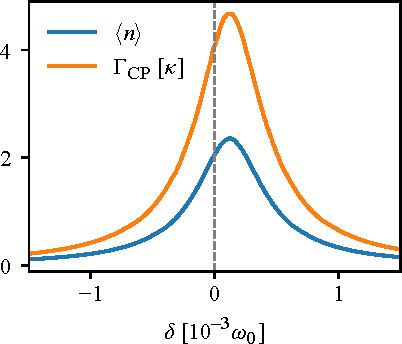
\includegraphics{jjcavity-photon-charge-plot.pdf}};
        \end{scope}

        \begin{scope}[shift={($(9cm,-6cm)$)}]
                \draw[-latex, thick] (0,0) -- (6.9,0) node[midway, below] {Cooper-pair number};
                \draw[-latex, thick] (0,0) -- (0,5.5)
                node[midway,left,label={[rotate=90]:Photon number}] {};

                
                        % Bottom
                        \draw[ultra thick] (1, 2) node[left, align=right] {$n-1$} -- (2, 2);
                        \draw[ultra thick] (3, 1.5) -- (4, 1.5) node[at start]
                        (N3) {} node[at end] (N10) {};
                        \draw[dashed] (4, 1.5) -- (6,1.5) node[at end, inner sep=0pt] (b) {};
                        \draw[ultra thick] (5, 1) -- (6, 1) node[at end, inner sep=0pt] (a) {};

                        \draw[ultra thick] (1, 3) node[left, align=right]
                        {$n$} -- (2, 3) node[at end] (N1) {};
                        \draw[ultra thick] (3, 2.5) -- (4, 2.5) node[at start]
                        (N2) {} node[at end] (N7) {};
                        \draw[ultra thick] (5, 2) -- (6, 2) node[at end, inner sep=0pt] (c) {};;

                        \draw[ultra thick] (1, 4) node[left, align=right]
                        {$n+1$} -- (2, 4);
                        \draw[ultra thick] (3, 3.5) -- (4, 3.5) node[at start]
                        (N4) {} node[at end] (N6) {};
                        \draw[ultra thick] (5, 3) node (N5) {} -- (6, 3) node[at end, inner sep=0pt] (d) {};

                        % Top
                        \draw[ultra thick] (1, 5) node[left, align=right]
                        {$n+2$} -- (2, 5);
                        \draw[ultra thick] (3, 4.5) -- (4, 4.5) node[at start]
                        (N8) {} node[at end] (N9) {};
                        \draw[ultra thick] (5, 4) -- (6, 4) node[at end, inner sep=0pt] (e) {};

                        \node at (1.5, 0.5) {$N$};
                        \node at (3.5, 0.5) {$N+1$};
                        \node at (5.5, 0.5) {$N+2$};

                        % Arrows
                        \draw[<->, >=latex] (a) -- (b) node[midway, right] {$\omega_J$};
                        \draw[<->, >=latex] (b) -- (c) node[midway, right]
                        {$\omega_J$};
                        \draw[<->, >=latex, ultra thick] (d) -- (e) node[midway, right]
                        {$\omega_0$};

                        \draw[->, >=stealth, ultra thick, red] (N1) -- (N2);
                        \draw[->, >=stealth, ultra thick, red] (N1) -- (N4);
                        \draw[->, >=stealth, ultra thick, red] (N6) -- (N5);
                        \draw[->, >=stealth, ultra thick, red] (N7) -- (N5);

                        \draw[->, >=stealth, ultra thick, red!50] (N1) -- (N3);
                        \draw[->, >=stealth, ultra thick, red!50] (N1) -- (N8);
                        \draw[->, >=stealth, ultra thick, red!50] (N9) -- (N5);
                        \draw[->, >=stealth, ultra thick, red!50] (N10) -- (N5);
                

        \end{scope}

\end{tikzpicture}

\end{document} 
